\section{XML message types} \label{sec:xml}

\vspace{-20pt}\hspace{180pt}
\difxoneone

\vspace{7pt}

The {\tt difxmessage} library (\S\ref{sec:difxmessage}) implements a system for sending and receiving messages using XML format.
This section documents the ``difxMessage'' XML document type that is used for interprocess communication during correlation within DiFX.
These messages are sent via UDP multicast and are thus restricted to fit within one standard-sized Ethernet packet ($\sim$1500 bytes).
Various logging and monitoring programs ({\tt mk5mon}, {\tt cpumon}, and {\tt errormon}, all eventually to be replaced by a single interactive operator interface) can accept these messages and perform actions based on their content.
Several different message types are derived from the following XML base type:

\begin{quotation}
\begin{Verbatim}[commandchars=\|\[\]]
<?xml version="1.0" encoding="UTF-8"?>
<difxMessage>
  <header>
    <from>|bfit[from]</from>
    <to>|bfit[to]</to>
    <mpiProcessId>|bfit[mpiId]</mpiProcessId>
    <identifier>|bfit[idString]</identifier>
    <type>|bfit[messageType]</type>
  </header>
  <body>
    <seqNumber>|bfit[seqNum]</seqNumber>
    |bfit[body]
  </body>
</difxMessage>
\end{Verbatim}
\end{quotation}

\noindent The italicized fields are as follows:

\begin{description}

\item[\bfit{from}] the hostname of the sender.
\item[\bfit{to}] the intended recipient of the XML document.
Note that this field is typically not included for report-only messages as it's intended purpose is for directing commands to particular recipients.
Also note that multiple \bfit{to} fields can be present in a message.
Three ``shortcuts'' are currently allowed: {\tt all} causes all receiving programs (such as {\tt mk5daemon}) on all software correlator cluster members to respond; {\tt mark5} causes all Mark5 units to respond; and {\tt swc} causes all non-Mark5 units to respond.
\item[\bfit{mpiId}] the MPI process id of the sender.  
If there are $D$ (typically 10) datastream processes (i.e., Mark5 units playing back), then \bfit{mpiId} takes on the following numbers:

\begin{tabular}{cl}
value    & {\tt mpifxcorr} process type \\
\hline
$< 0$    & a process not associated with {\tt mpifxcorr} \\
$0$      & the manager process of {\tt mpifxcorr} \\
1 to $D$ & one of the datastream processes \\
$\ge D+1$  & one of the core (computing) processes 
\end{tabular}

\item[\bfit{idString}] an additional string identifying the source of the message.  
For messages sent from {\tt mpifxcorr}, this will be the job id, for example {\tt job3322.000}.  
Other programs will typically set this field to the name of the program sending the message. 
\item[\bfit{messageType}] the type of message being sent:

\begin{tabular}{ll}
value    & description of message type \\
\hline
{\tt DifxAlertMessage} & an error message. \\
{\tt DifxCommand} & a command message. \\
{\tt DifxLoadMessage} & CPU and memory usage (usually sent by {\tt mk5daemon}). \\
{\tt DifxParameterMessage} & specify new parameter value to an {\tt mpifxcorr} process. \\
{\tt DifxStartMessage} & tell head node to start a difx job. \\
{\tt DifxStopMessage} & tell {\tt mk5daemon} to stop a particular instance of {\tt mpifxcorr}. \\
{\tt DifxStatusMessage} & status of the {\tt mpifxcorr} program. \\
{\tt Mark5ConditionMessage} & Mark5 module conditioning statistics for one disc. \\
{\tt Mark5StatusMessage} & status of the mark5 unit and modules. \\
{\tt Mark5VersionMessage} & versions, board types and serial numbers of a Streamstor card. 
\end{tabular}

\noindent Each of these message types is described in sections that follow.

\item[\bfit{seqNum}] the sequence number (starting at 0) of messages coming from the particular program running on the particular host.
The number advances by 1 for each sent message and can be used to detect lost packets.
\item[\bfit{body}] message contents that are specific to the particular \bfit{messageType}.
See sections that follow.
\end{description}

A ``C'' language library for generating, multicasting, receiving, and parsing XML documents of this type is used within some of the programs, including {\tt mpifxcorr} (the core of the DiFX \cite{difx} software correlator) and {\tt mk5daemon} (a program that runs on each Mark5 unit that is responsible for multicast communication when {\tt mpifxcorr} is not running), that transact these XML documents.
The default multicast group to be used is 224.2.2.1 and the default port is 50200, though these can be overridden with environment variables {\tt DIFX\_MESSAGE\_GROUP} and {\tt DIFX\_MESSAGE\_PORT} respectively.






% DifxAlertMessage ------------------------------------------------------------

\subsection{DifxAlertMessage} \label{sec:difxalertmessage}

This section describes messages with \bfit{messageType} = {\tt DifxAlertMessage}.
These messages come from mpifxcorr or the head node agent and contain an error message string and severity code that should be displayed to the operator and logged.

The \bfit{body} of the message contains:

\begin{quotation}
\begin{Verbatim}[commandchars=\|\[\]]
    <difxAlert>
      <alertMessage>|bfit[message]</alertMessage>
      <severity>|bfit[severity]</severity>
    </difxAlert>
\end{Verbatim}
\end{quotation}


\noindent The italicized fields are as follows:

\begin{description}
\item{\bfit{message}} a string containing the error message.
\item{\bfit{severity}} an integer indicating the severity. 
The severity scale is based on that from the EVLA and has values with the following meanings:

\begin{tabular}{cll}
value    & name & meaning \\
\hline
0 & FATAL   & processing has failed; a restart is needed  \\
1 & SEVERE  & data from one or more station is affected badly \\
2 & ERROR   & data from one or more station may be affected; e.g., low weights \\
3 & WARNING & minor error of no consequence to ongoing processing \\
4 & INFO    & informational only \\
5 & VERBOSE & overly verbose infomation \\
6 & DEBUG   & debugging information 
\end{tabular}

\end{description}






% DifxCommand -----------------------------------------------------------------

\subsection{DifxCommand}

This section describes messages with \bfit{messageType} = {\tt DifxCommand}.
These messages require the \bfit{to} field to be set and cause the intended recipient to take an action.

The \bfit{body} of the message contains:

\begin{quotation} 
\begin{Verbatim}[commandchars=\|\[\]] 
    <difxCommand>
      <command>|bfit[command]</command>
    </difxCommand>
\end{Verbatim}
\end{quotation}

\noindent The italicized field is as follows:

\begin{description}
\item{\bfit{command}} the command to execute.
Commands are not case sensitive and should be among the following:

\begin{tabular}{ll}
command & action\\
\hline
{\tt GetVSN} & cause the mark5 unit to multicast loaded VSNs if possible. \\
{\tt GetLoad} & request CPU and memory usage to be reported. \\
{\tt ResetMark5} & cause {\tt SSReset} and {\tt ssopen} to be run to reset Streamstor. \\
{\tt StartMark5A} & start the Mark5A program. \\
{\tt StopMark5A} & stop the Mark5A program. \\
{\tt KillMpifxcorr} & kill with signal 9 (sigkill) any process with name {\tt mpifxcorr}. \\
{\tt Clear} & reset the mk5daemon; useful sometimes if {\tt mpifxcorr} crashes. \\
{\tt Reboot} & causes machine to reboot. \\
{\tt Poweroff} & causes machine to power down. \\
{\tt Copy <bank> <vsn> <scans>} & causes scans to be copied to local disk. \\
\end{tabular}






% DifxLoadMessage -------------------------------------------------------------

\subsection{DifxLoadMessage}

This section describes messages with \bfit{messageType} = {\tt DifxLoadMessage}.
These messages contain CPU and memory utilization information and are voluntarily sent by various nodes of the cluster, to be received by the operator interface.

The \bfit{body} of this message type contains:

\begin{quotation}
\begin{Verbatim}[commandchars=\|\[\]]
    <difxLoad>
      <cpuLoad>|bfit[cpuLoad]</cpuLoad>
      <totalMemory>|bfit[totalMemory]</totalMemory>
      <usedMemory>|bfit[usedMemory]</usedMemory>
    </difxLoad>
\end{Verbatim}
\end{quotation}

\noindent The italicized fields are as follows:

\begin{description}
\item{\bfit{cpuLoad}} CPU utilization on the cluster node.  
It is a floating point value containing the average number of processes scheduled at one time.
\item{\bfit{totalMemory}} total memory on node, in kiB.
\item{\bfit{usedMemory}} used memory on node, in kiB.
\end{description}






% DifxParameter ---------------------------------------------------------------

\subsection{DifxParameter}

\begin{quotation} 
\begin{Verbatim}[commandchars=\|\[\]] 
    <difxParameter>
      <targetMipId>|bfit[id]</targetMpiId>
      <name>|bfit[name]</name>
      <index1>|bfit[index1]</index1>
      .
      .
      .
      <indexN>|bfit[indexN]</indexN>
      <value>|bfit[value]</value>
    </difxParameter>
\end{Verbatim}
\end{quotation}

Such a message is intended to allow a parameter, possibly qualified with array indices, to be set to a particular value.

\noindent The italicized fields are as follows:

\begin{description}
\item{\bfit{targetMpiId}} the MPI process Id (rank) to target with this message.
Values zero and greater target specific MPI processes, with zero always being the manager process.
Other special values include:

\begin{tabular}{ll}
value & meaning \\
\hline
-1 & all MPI processes \\
-2 & all core (processing) processes \\
-3 & all datastream processes \\
\end{tabular}

\item{\bfit{name}} the name of the parameter to set.
For array types, the following \bfit{index} values specify the element to set.
\item{\bfit{index}{\it N}} an integer specifying the index of the particular array axis.
\item{\bfit{value}} a string containing the value.

\end{description}






% DifxTransientMessage -------------------------------------------------------------

\subsection{DifxTransientMessage}

This section describes messages with \bfit{messageType} = {\tt DifxTransientMessage}.
This message is related to a commensal transient search project.
A message of this type should be sent as soon as possible after detection; it is likely that no provisions will be made for data copying that does not start before resources assigned to the job are released.
When a possible transient is identfied by a detecting program which looks at autocorrelations it sends this message to all Mark5 units.  
Once correlation is complete, the {\tt mk5daemon} program on appropriate Mark5 units will take a few seconds to copy data from the time range(s) of interest.

The \bfit{body} of this message type contains:

\begin{quotation}
\begin{Verbatim}[commandchars=\|\[\]]
    <difxTransient>
      <jobId>|bfit[jobId]</jobId>
      <startMJD>|bfit[startMJD]</startMJD>
      <stopMJD>|bfit[stopMJD]</stopMJD>
      <priority>|bfit[priority]</priority>
      <destDir>|bfit[destDir]</destDir>
      <comment>|bfit[comment]</comment>
    </difxTransient>
\end{Verbatim}
\end{quotation}

\noindent The italicized fields are as follows:

\begin{description}
\item{\bfit{jobId}} The job indentification string.
This is required so that only relevant Mark5 units take action on the received message.
\item{\bfit{eventId}} A string containing the name of the event as declared by the transient detector.
\item{\bfit{startMJD}} The start time (MJD) of the segment of data to copy.
\item{\bfit{stopMJD}} The stop time (MJD) of the segment of data to copy.
Note that the total amount of data to be copied should be low enough to have an inconsequential impact on correlation throughput.
\item{\bfit{priority}} A floating point value indicating the relative importance of capturing this event.
In jobs where many triggers occur this field will be used to select the most important ones to save to disk.
Higher numbers indicate higher priority.
\item{\bfit{destDir}} (optional) A final directory to store the baseband data.
If not provided, a default will be assumed.
Note that behavior is undefined if different destination directories are provided within a single job.
\item{\bfit{classification}} (optional) A string provided by the transient detector containing a tentative classification.
\item{\bfit{comment}} (optional) A comment that could be appended to a log file.
\end{description}

All data and a log file will be stored in a subdirectory of the data staging area named \bfit{jobId}.
The log file, at a minimum, will contain the list of events sent by the transient detection program and a log of the copying process, indicating any errors that may have occured.
The subdirectory will have a temporary name starting with a period ({\tt .}) until all data copy for the job in question is complete.
The use of this message type is demonstrated in Fig.~\ref{fig:transient}.

\begin{figure}[h]
\begin{center}
\resizebox{4in}{!}{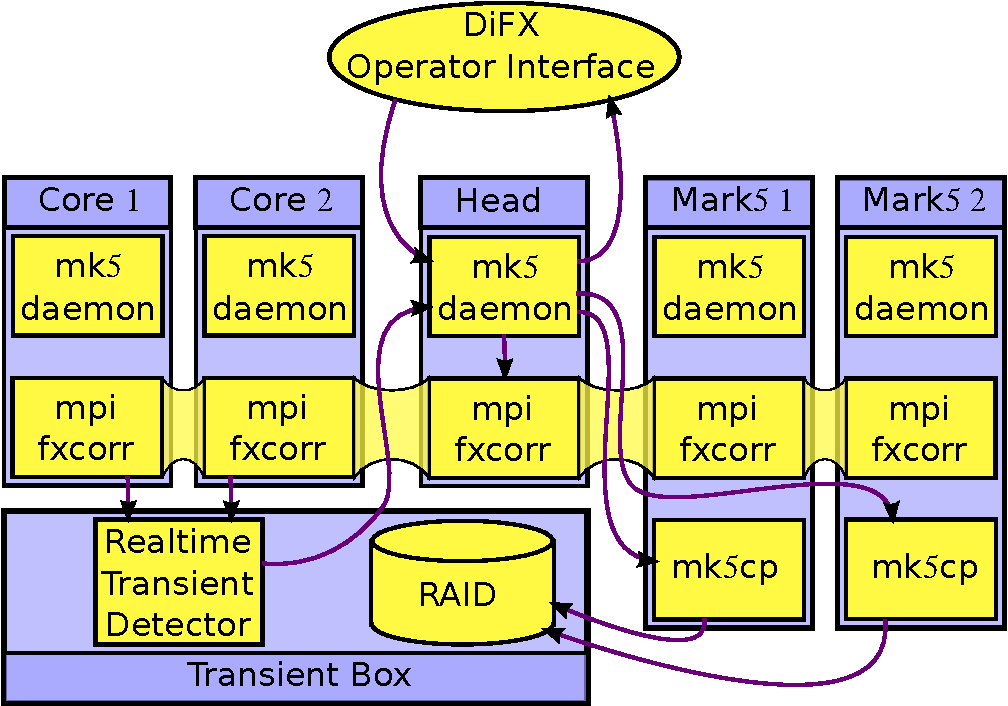
\includegraphics{transient}}
\caption[blockdiagram]{
{{\em The sequence of events leading to transient data capture.}
First the DiFX Operator Interface sends a {\tt DifxStart} message to the head node, causing the {\tt mpifxcorr} process to be started.
The core nodes of {\tt mpifxcorr} will transmit autocorrelation data to a real-time transient detection algorithm.
As interesting events are identified, {\tt DifxTransientMessage} documents are sent to the head node; the {\tt mk5daemon} process keeps a prioritized list of events.
After correlation completes but before {\tt mk5daemon} on the head node starts a series of {\tt mk5cp} processes to run to copy the baseband data from the Mark5 modules before the next job starts.
}
\label{fig:transient}
}
\end{center}
\end{figure}





% DifxStart -------------------------------------------------------------------

\subsection{DifxStart}

This document type causes the head node to spawn a correlator job.
The doument contents describe which resources to use and which {\tt .input} file to use.

The \bfit{body} of the message contains:

\begin{quotation}
\begin{Verbatim}[commandchars=\|\[\]]
    <difxStart>
      <input>|bfit[input file]</input>
      <force>|bfit[forceOverwrite]</force>
      <manager node="|bfit[node]" />
      <datastream nodes="|bfit[nodes]" />
      <process nodes="|bfit[nodes]" threads="|bfit[count]" />
      <env>|bfit[envvar]=|bfit[value]</env>
      <difxProgram>|bfit[program]</difxProgram>
      <difxVersion>|bfit[version]</difxVersion>
      <mpiWrapper>|bfit[mpiWrapper]</mpiWrapper>
      <mpiOptions>|bfit[options]</mpiOptions>
    </difxStart>
\end{Verbatim}
\end{quotation}

In the above XML file, exactly one manager node must be supplied.
There must be at least one datastream node (one per antenna being correlated).
There must be at least one process node.
Zero or more (up to a maximum of 8) environment variables may be set.
The italicized fields are as follows:

\begin{description}
\item{\bfit{input file}} complete path to the {\tt .input} file for this correlation.
\item{\bfit{forceOverwrite}} cause any previous correlator output of this job to be deleted before starting the correlation.  A value of {\tt 1} or {\tt True} will enable overwrite.
\item{\bfit{value}} the value of the environment variable.
\item{\bfit{node}} the name of the node being assigned, e.g. {\tt mark5fx02} or {\tt swc000}.
\item{\bfit{nodes}} a list of node names.  The list members should be space or comma separated.
\item{\bfit{count}} the maximum number of threads to schedule.  If not specified, 1 will be assumed.
This applies only to process nodes.
\item{\bfit{envvar}} an environment variable to set before running mpifxcorr.
\item{\bfit{program}} the name of the software correlator executable.
This is optional and defaults to {\tt mpifxcorr} if not set.
\item{\bfit{version}} the version (e.g., {\em DIFX-1.5.4}) of DiFX to run.
\item{\bfit{mpiWrapper}} the name of the program used to start the MPI processes.
This field is optional and defaults to {\tt mpirun} if none is provided.
\item{\bfit{options}} extra options to pass to {\tt mpirun}.
This is optional; sensible defaults are assumed if not explicitly set.
\end{description}

Note that multiple {\tt <process />} tags can be specified, each with its own thread count.
Each tag's thread count only affects those nodes specified in that tag.
If {\bfit{version}} is provided, then a wrapper script called {\tt runmpifxcorr.}{\em version} is expected to be in the default path which sets the environment for the version of DiF to actuallyt run.





% DifxStatusMessage -----------------------------------------------------------

\subsection{DifxStatusMessage}

This section describes messages with \bfit{messageType} = {\tt DifxStatusMessage}.
This message type is only produced by {\tt mpifxcorr} or the programs immediately responsible for starting and stopping it.

The \bfit{body} of the message contains:

\begin{quotation}
\begin{Verbatim}[commandchars=\|\[\]]
    <difxStatus>
      <state>|bfit[state]</state>
      <message>|bfit[message]</message>
      <visibilityMJD>|bfit[visibilityMJD]</visibilityMJD>
      <weight ant=|bfit[antId] wt=|bfit[weight]>
    </difxStatus>
\end{Verbatim}
\end{quotation}

\noindent The italicized fields are as follows:

\begin{description}
\item{\bfit{state}} the state of {\tt mpifxcorr}, which must be one of the following:

\begin{tabular}{ll}
state & meaning \\
\hline
{\tt Spawning} & the {\tt mpifxcorr} processes are being started (not sent by {\tt mpifxcorr}).\\
{\tt Starting} & all the processes are ready to begin. \\
{\tt Running} & the correlator is running. \\
{\tt Ending} & the correlator has reached the end of the job. \\
{\tt Done} & the correlation has completed. \\
{\tt Aborting} & correlation is stopping early due to an error. \\
{\tt Terminating} & correlation is stopping early due to signal. \\
{\tt Terminated} & correlation has stopped early. \\
{\tt MpiDone} & all of the MPI processes have ended (not sent by {\tt mpifxcorr}). \\
{\tt Crashed} & {\tt mpifxcorr} crashed; usually sent by {\tt mk5daemon}.
\end{tabular}

\item{\bfit{message}} a string containing information for the operator.
\item{\bfit{visibilityMJD}} the time-stamp (MJD + fraction) of last completed visibility record.
\item{\bfit{antId}} the antenna id for the associated weight, ranging from 0 to $N_{\mathrm{ant}}-1$.
\item{\bfit{weight}} the data weight for the associated antenna, ranging from 0 to 1.
Note that in each XML document of this type there will in general be one \bfit{weight} value for each antenna being correlated.
\end{description}







% DifxStop ------------------------------------------------ INCOMPLETE? -------

\subsection{DifxStop}

Messages with \bfit{messageType} = {\tt DifxStop} are typically sent by the DiFX Operator Interface to the {\tt mk5daemon} running on the correlator head node to cause a particular instance of DiFX to be killed.

The \bfit{body} of the message contains:

\begin{quotation}
\begin{Verbatim}[commandchars=\|\[\]]
    <difxStop>
    </difxStop>
\end{Verbatim}
\end{quotation}





% Mark5ConditionMessage -------------------------------------------------------

\subsection{Mark5ConditionMessage}

Mark5 module conditioning is done periodically to ensure top performance of Mark5 modules.
Each disk in the module gets written across its whole surface to identify bad areas and to {\em calibrate} the electronics.
One message applies to one disk of the module

The \bfit{body} of the message contains:

\begin{quotation}
\begin{Verbatim}[commandchars=\|\[\]]
    <difxCondition>
      <serialNumber>|bfit[serial]</serialNumber>
      <modelNumber>|bfit[model]</modelNumber>
      <size>|bfit[size]</size>
      <moduleVSN>|bfit[vsn]</moduleVSN>
      <moduleSlot>|bfit[slot]</moduleSlot>
      <startMJD>|bfit[startMJD]</startMJD>
      <stopMJD>|bfit[stopMJD]</stopMJD>
      <bin|bfit[N]>|bfit[statsN]</bin|bfit[N]>
    </difxCondition>
\end{Verbatim}
\end{quotation}

\noindent The italicized fields are as follows:

\begin{description}
\item{\bfit{serial}} the serial number of the disk.
\item{\bfit{model}} the model number of the disk.
\item{\bfit{size}} the size of the disk, in GB.
\item{\bfit{vsn}} the module Volume Serial Number (VSN).
\item{\bfit{slot}} the location of the disk within the module, from 0 to 7.
\item{\bfit{startMJD}} the time when conditioning began.
\item{\bfit{stopMJD}} the time when condtioning ended.
\item{\bfit{statsN}} the histogram count for bin \bfit{N} for \bfit{N} in the range 0 to 7.
\end{description}







% Mark5StatusMessage ----------------------------------------------------------

\subsection{Mark5StatusMessage}

This section describes messages with \bfit{messageType} = {\tt Mark5StatusMessage}.
This message type cones from either {\tt mpifxcorr} or {\tt mk5daemon} (or perhaps another program that makes heavy use of Mark5 units and wishes to volunteer status information).

The \bfit{body} of the message contains:

\begin{quotation}
\begin{Verbatim}[commandchars=\|\[\]]
    <mark5Status>
      <bankAVSN>|bfit[vsnA]</bankAVSN>
      <bankBVSN>|bfit[vsnB]</bankBVSN>
      <statusWord>|bfit[statusWord]</statusWord>
      <activeBank>|bfit[activeBank]</activeBank>
      <state>|bfit[state]</state>
      <scanNumber>|bfit[scanNumber]</scanNumber>
      <scanName>|bfit[scanName]</scanName>
      <position>|bfit[position]</position>
      <playRate>|bfit[playRate]</playRate>
      <dataMJD>|bfit[dataMJD]</dataMJD>
    </mark5Status>
\end{Verbatim}
\end{quotation}

\noindent The italicized fields are as follows:

\begin{description}
\item{\bfit{vsnA}} the VSN of the module in bank A.
\item{\bfit{vsnB}} the VSN of the module in bank B.
\item{\bfit{statusWord}} a hexadecimal number with the following bits:
{\em TBD}
\item{\bfit{activeBank}} the active bank, either {\tt A} or {\tt B} for banks A and B respectively, {\tt N} if the unit is in non-bank mode, or blank if no modules are active.
\item{\bfit{state}} the state of the Mark5 unit:

\begin{tabular}{ll}
state & meaning \\
\hline
{\tt Opening} & the Streamstor card is being opened. \\
{\tt Open} & the Streamstor was successfully opened and is ready for use. \\
{\tt Close} & the Streamstor has been closed. \\
{\tt GetDirectory} & the unit is recovering the directory or finding data. \\
{\tt GotDirectory} & the unit successfully found needed data on the module. \\
{\tt Play} & the unit is playing back data. \\
{\tt PlayStart} & the unit is about to start playback. \\
{\tt PlayInvalid} & the unit is playing data, but the data is invalid. \\
{\tt Idle} & the unit is not doing anything; no process has control of it. \\
{\tt Error} & the unit is unusable due to an error. \\
{\tt Busy} & the unit is busy and cannot respect commands. \\
{\tt Initializing} & the Streamstor card is initializing. \\
{\tt Resetting} & the unit is resetting the Streamstor card. \\
{\tt Rebooting} & the unit is about to reboot. \\
{\tt Poweroff} & the unit is about to turn off. \\
{\tt NoData} & the unit is not playing data since there is none that is appropriate. \\
{\tt NoMoreData} & the unit has played all the data for the job and is stopped. \\
{\tt Copy} & data is being copied off the module to a local disk. \\
\end{tabular}

\item{\bfit{scanNumber}} the directory index number for the current scan.
This number starts at 1.
\item{\bfit{scanName}} the name associated with the current scan.
\item{\bfit{position}} the byte position being accessed. 
Note that this number can be very large ($> 2^{46}$).
\item{\bfit{playRate}} the time-averaged playback rate in Mbps.
\item{\bfit{dataMJD}} the date stamp (MJD + fraction) of the most recently read data.
\end{description}







% Mark5VersionMessage ---------------------------------------------------------

\subsection{Mark5VersionMessage} % new

This section describes messages with \bfit{messageType} = {\tt Mark5VersionMessage}.
This message comes from {\tt mk5daemon}.
It is typically broadcast once upon the start of {\tt mk5daemon} and when requested.

The \bfit{body} of the message contains:

\begin{quotation}
\begin{Verbatim}[commandchars=\|\[\]]
    <mark5Version>
      <ApiVer>|bfit[ApiVer]</ApiVer>
      <ApiDate>|bfit[ApiDate]</ApiDate>
      <FirmVer>|bfit[FirmVer]</FirmVer>
      <FirmDate>|bfit[FirmDate]</FirmDate>
      <MonVer>|bfit[MonVer]</MonVer>
      <XbarVer>|bfit[XbarVer]</XbarVer>
      <AtaVer>|bfit[AtaVer]</AtaVer>
      <UAtaVer>|bfit[UAtaVer]</UAtaVer>
      <DriverVer>|bfit[DriverVer]</DriverVer>
      <BoardType>|bfit[BoardType]</BoardType>
      <SerialNum>|bfit[SerialNum]</SerialNum>
      <DaughterBoard>
        <PCBType>|bfit[PCBType]</PCBType>
        <PCBSubType>|bfit[PCBSubType]</PCBSubType>
        <PCBVer>|bfit[PCBVersion]</PCBVer>
        <FPGAConfig>|bfit[FPGAConfig]</FPGAConfig>
        <FPGAConfigVer>|bfit[FPGAConfigVersion]</FPGAConfigVer>
      </DaughterBoard>
    </mark5Version>
\end{Verbatim}
\end{quotation}


\noindent Note that the {\tt DaughterBoard} tag and its subtags are optional and are not broadcast if a daughter board is not detected on the Mark5C unit.
The italicized fields are as follows:

\begin{description}
\item{\bfit{ApiVer}} The software API version of the Streamstor API.
\item{\bfit{ApiDate}} Date associated with the above.
\item{\bfit{FirmVer}} The version of the firmware that is loaded.
\item{\bfit{FirmDate}} Date associated with the above.
\item{\bfit{MonVer}} The version of the Monitor FPGA code.
\item{\bfit{XbarVer}} The version of the cross bar FPGA code
\item{\bfit{AtaVer}} The version of the ATA disk controller FPGA code.
\item{\bfit{UAtaVer}} The version of the UATA disk controller FPGA code.
\item{\bfit{DriverVer}} The version number of the driver code.
\item{\bfit{BoardType}} The type of Streamstor board.
\item{\bfit{SerialNum}} The serial number of the Streamstor board.
\item{\bfit{PCBType}} The type of Streamstor daughter board.
\item{\bfit{PCBSubType}} Subtype of the above, if any.
\item{\bfit{PCBVersion}} The version of the daughter board.
\item{\bfit{FPGAConfig}} Name of the FPGA configuration.
\item{\bfit{FPGAConfigVersion}} Version number of FPGA configuration.
\end{description}


\end{description}

